\documentclass[12pt, a4paper]{article}

\usepackage[utf8]{inputenc}
\usepackage[russian]{babel}
\usepackage{geometry}
\usepackage{mathtools}
\usepackage{verbatim}
\usepackage{indentfirst}
\usepackage{caption}
\usepackage{subcaption}
\usepackage{import}
\usepackage{xifthen}
\usepackage{pdfpages}
\usepackage{transparent}
\usepackage{graphicx}
\usepackage{caption}
\usepackage{hyperref}
\usepackage{float}

\newcommand{\norm}[1]{\lVert #1 \rVert}
\newcommand{\abs}[1]{\lvert #1 \rvert}
\usepackage[oglav,spisok,boldsect,eqwhole,figwhole,hyperref,hyperprint,remarks,greekit]{./style/fn2kursstyle}

\graphicspath{{./style/}{./figures/}}

\frenchspacing

\title{Методы численного решения обыкновенных дифференциальных уравнений}
\lab{1}
\author{М.\,А.~Каган}
\creator{И.\,А.~Яковлев}
\supervisor{}
\group{ФН2-61Б}
\date{2025}

\begin{document}
	\maketitle
	\tableofcontents
	
	\newpage
	
	
	
	\section-{Контрольные вопросы}
	
	\begin{enumerate}
		\item \textbf{Сформулируйте условия существования и единственности решения задачи Коши для обыкновенных дифференциальных уравнений. Выполнены ли они для вашего варианта задания?}
		\vspace*{0.2cm}
		
		\textit{\textbf{Ответ:}}
		
		Рассмотрим векторную функцию $u: I \subseteq \mathbb{R} \rightarrow \mathbb{R}^n$, где $t \in \mathbb{R}$. Рассмотрим задачу Коши:

		\[
		\begin{cases}
			u' = f(t, u) \\
			u(t_0) = u_0 \\
		\end{cases}
		\]
		\begin{enumerate}
			\item Пусть функция  $f(t, u)$ определена и непрерывна в прямоугольнике:
			\[
			D = \Bigl\{ (t, u): |t - t_0| \le a; |u_i - u_{0, i}| \le b \Bigr\}.
			\]
			Выберем $M > 0$, такую что $|f_i| < M$.
			\item Пусть функция $f(t, u)$ липшиц-непрерывна с постоянной $L$ по переменным $u_1, u_2, \ldots, u_n$:
			\[
			|f(t, u^{(1)}) - f(t, u^{(2)})| \le L\sum\limits^{n}_{i=1}|u^{(1)} - u^{(2)}|
			\]
		\end{enumerate}
		
		Тогда решение задачи Коши существует и единственно на участке
		\[
		|t - t_0| \le \min{a, b/M, 1/L}
		\]
		
		\item \textbf{Что такое фазовое пространство? Что называют фазовой траекторией? Что называют интегральной кривой?}
		\vspace*{0.2cm}
		
		\textit{\textbf{Ответ:}}

		Решение дифференциального уравнения (или системы дифференциальных уравнений) $X = X(t)$ можно интерпретировать геометрически как кривую в евклидовом пространстве $(t, \, x_1, \dots, \,x_n)$, где $t$ --- координата времени, $x_k$ --- координаты $n$-мерного пространства. Такая кривая называется интегральной кривой.

		Пространство $(x_1, \dots, \, x_n)$ называют фазовым пространством, кривую $X = X(t)$ --- фазовой траекторией.
		
		\item \textbf{Каким порядком аппроксимации и точности обладают методы, рассмотренные в лабораторной работе?}
		\vspace*{0.2cm}
		
		\textit{\textbf{Ответ:}}
		
		\begin{enumerate}
			\item Метод Эйлера:
			\begin{gather}
				\text{Порядок точности:}\;\; O(\tau)  \notag\\
				\text{Порядок Аппроксимации:}\;\; O(\tau) \notag
			\end{gather}
			\item Метод Рунге -- Кутты:
			\begin{gather}
				\text{Порядок точности:}\;\; O(\tau^4)  \notag\\
				\text{Порядок Аппроксимации:}\;\; O(\tau^4) \notag
			\end{gather}
			Замечание: порядок точности метода Рунге -- Кутты совпадает с его порядком аппроксимации
			\item Метод Адамса -- Башфорта:
			\begin{gather}
				\text{Порядок точности:}\;\; O(\tau^4)  \notag\\
				\text{Порядок Аппроксимации:}\;\; O(\tau^4) \notag
			\end{gather}
			Замечание: для обеспечения порядка аппроксимации порядка $p$ должны выполнятся $p+1$ уравнений
			\[
			\sum\limits^{m}_{k=0}\dfrac{1}{\tau}a_k = 0,\;\;\sum\limits^{m}_{k=0}k^{l-1}(b_k + a_k \dfrac{k}{l})=0,\;\;l=1, 2, \ldots, p
			\]
			и условие нормировки
			\[
			\sum\limits_{k=0}^{m} b_k = 1
			\]
			где линейный m-шаговый разностный метод:
			\[
			\dfrac{a_0 y_n + a_1 y_{n-1} + \ldots + a_m y_{n-m}}{\tau} = b_0 f_n + b_1 f_{n-1} + \ldots + b_m f_{n-m}
			\]
			\item Метод <<предиктор -- корректор>>:
			\begin{gather}
				\text{Порядок точности:}\;\; O(\tau^4)  \notag\\
				\text{Порядок Аппроксимации:}\;\; O(\tau^4) \notag %TODO: найти порядок аппроксимации
			\end{gather}
		\end{enumerate}
		
		\item \textbf{Какие задачи называются жесткими? Какие методы предпочтительны для их решения? Какие из рассмотренных методов можно использовать для решения жестких задач?}
		\vspace*{0.2cm}
		
		\textit{\textbf{Ответ:}}

		Система обыкновенных дифференциальных уравнений $u' = Au$ с постоянной матрицей $A$ размерности $n$ называется жесткой, если: 
		\begin{enumerate}
			\item все собственные значения матрицы $A$ имеют отрицательную действительную часть $Re \, \lambda_i < 0, \, i = \overline{1, \,n}$
			\item число жесткости $S$ системы велико, $S = \dfrac{\max \abs{Re \, \lambda_i}}{\min \abs{Re \, \lambda_i}} \gg 1$.
		\end{enumerate} 

		Особенность жестких задач состоит в том, что искомая функция изменяется достаточно медленно, и при увеличении шага возникает быстрое накопление погрешности. Поэтому необходимо использовать устойчивые методы, по отношению к жестким задачам A-устойчивые или $A(\alpha)-$устойчивые, т.е. устойчивые в левой полуплоскоти $Re \, \mu < 0$ или ее секторе $\alpha$.

		К таким методам относятся, например, неявный метод Эйлера и симметричная схема, а также метод Гира.
		
		\item \textbf{Как найти $\vec{y}_1$, $\vec{y}_2$, $\vec{y}_3$, чтобы реализовать алгоритм прогноза и коррекции (1.18)?}
		\vspace*{0.2cm}
		
		\textit{\textbf{Ответ:}}
		
		\begin{enumerate}
			\item Воспользоваться одношаговым явным методом, например, Рунге -- Кутты 4-го порядка для нахождения первых 3 значений $y$.
			\item Разложить искомую функцию в ряд Тейлора в точке $t_0$ или экстраполировать каким либо другим способом. 
		\end{enumerate}
		
		\item \textbf{ Какой из рассмотренных алгоритмов является менее трудоемким? Какой из рассмотренных алгоритмов позволяет достигнуть заданную точность, используя наибольший шаг интегрирования? Какие достоинства и недостатки рассмотренных алгоритмов вы можете указать?}
		\vspace*{0.2cm}
		
		\textit{\textbf{Ответ:}}

		Съ точкиъ зренияъ банальной эрудицииъ, \textbf{явный метод Эйлера} является наименее трудоемким: на одной итерации требуется вызывать всего лишь один раз функцию правой части. Также обладает несложной реализацией. Однако имеет лишь первый порядок точности и не подходит для решения жестких задач.

		\textbf{Неявный метод Эйлера} также имеет первый порядок точности, но подходит для решения жестких задач. Однако в общем случае на каждом шаге необходимо решать систему нелинейных уравнений, что повышает трудоемкость.

		\textbf{Симметричная схема} является модификацией неявного метода Эйлера, повышающей порядок с первого до второго.

		\textbf{Метод Рунге-Кутты 4 порядка} обладает четвертым порядком сходимости и позволяет достигнуть наибольшую точность, используя наибольший шаг интегрирования, однако не подходит для решения жестких задач и трудоемок по количеству операций: на каждом шаге функция правой части вычисляется 4 раза.

		\textbf{Метод Адамса} имеет тот же порядок сходимости, что и метод Рунге-Кутты 4 порядка и при этом на одном шаге требует лишь один раз вычислять функцию правой части, однако также не подходит для решения жестких задач и требует реализации дополнительного метода решения ОДУ на первых трех шагах.

		\textbf{Метод <<предиктора-корректора>>} имеет 4 порядок точности, вычисляет функцию правой части 2 раза, но так как он основан на методе простой итерации, от функции требуются дополнительные условия для сходимости. Также требует реализации дополнительного метода решения ОДУ на первых трех шагах.
		
		%TODO: додумать
		\item \textbf{Какие алгоритмы, помимо правила Рунге, можно использовать для автоматического выбора шага?}
		\vspace*{0.2cm}
		
		\textit{\textbf{Ответ:}}
		\begin{enumerate}
			\item На каждые $k$ шагов линеаризовывать систему ДУ, оценивая сверху или численно находя собственное значение. Зная диапазон $\lambda \ge \max\limits_{i}\lambda_i$, где $\lambda_i$ собственные значения линеаризованной системы, будем выбирать шаг $\tau = \dfrac{1}{\lambda}$ 
			
			\item Для методов Рунге -- Кутты можно построить такие таблицы коэффициентов как на рис. \ref{fig:Special-Butcher}, 
			\begin{figure}[h]
				\centering
				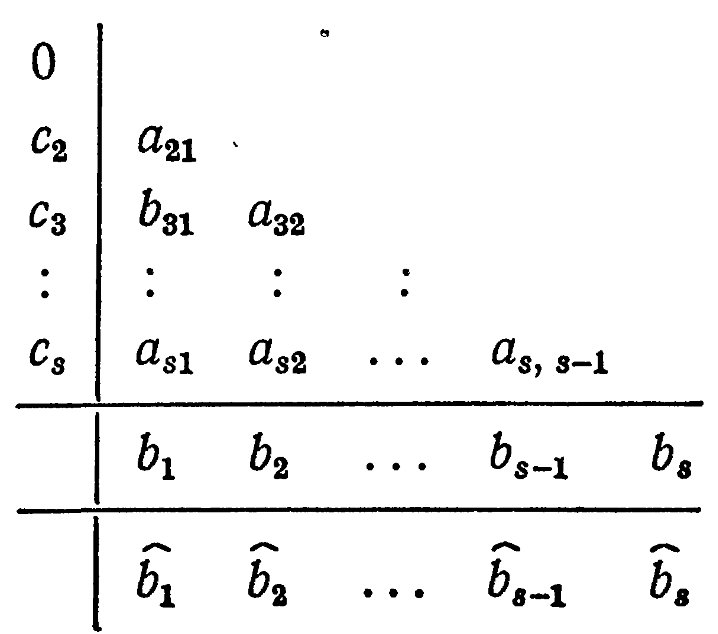
\includegraphics[width=0.6\textwidth]{butcher_table_sp}
				\caption{Таблица }
				\label{fig:Special-Butcher}
			\end{figure}
			 чтобы один из двух методов обладал порядком точности на 1 больше. Таким образом, из полученных значений $y_n$ и $\tilde{y_n}$ можно получить оценку погрешности аппроксимации, основываясь на которой необходимо увеличить или уменьшить шаг.
		\end{enumerate}
		
	\end{enumerate}

	
	
	
	
\end{document}